\documentclass[12pt,a4paper]{article}
\usepackage[ngerman]{babel}
\usepackage[utf8]{vietnam}
\usepackage{amsmath}
\usepackage{amsfonts}
\usepackage{amsthm}
\usepackage{listings}
\usepackage{lmodern}
\usepackage{amssymb}
\usepackage{graphicx}
\usepackage{xifthen}
\usepackage{float}
\usepackage{lastpage}
\usepackage{color}
\usepackage[table,xcdraw]{xcolor}
\usepackage{tabularx}
\usepackage{booktabs}

\usepackage[left=2cm,right=2cm,top=2cm,bottom=2cm]{geometry}
\usepackage{scrextend}
\usepackage{fancyhdr}
\pagestyle{fancy}
\lhead{Quy hoạch tuyến tính}
\rhead{Giữa kỳ}
\setcounter{tocdepth}{1}
%\renewcommand{\thefigure}{\arabic{section}.\arabic{figure}}

\newcommand{\oneline}[1]{%
  \newdimen{\namewidth}%
  \setlength{\namewidth}{\widthof{#1}}%
  \ifthenelse{\lengthtest{\namewidth < \textwidth}}%
  {#1}% do nothing if shorter than text width
  {\resizebox{\textwidth}{!}{#1}}% scale down
}

%\renewcommand\tabularxcolumn[1]{>{\centering\arraybackslash}m{#1}}
\newcolumntype{Z}[0]{>{\hsize=1.55\hsize}X}%
\newcolumntype{s}[0]{>{\hsize=.6\hsize}X}%
\newcolumntype{n}[0]{>{\centering\arraybackslash\hsize=1.25\hsize}X}

\definecolor{dkgreen}{rgb}{0,0.6,0}
\definecolor{gray}{rgb}{0.5,0.5,0.5}
\definecolor{mauve}{rgb}{0.58,0,0.82}

\lstset{frame=tb,
  language=Python,
  aboveskip=3mm,
  belowskip=3mm,
  showstringspaces=false,
  columns=flexible,
  basicstyle={\small\ttfamily},
  numbers=none,
  numberstyle=\tiny\color{gray},
  keywordstyle=\color{blue},
  commentstyle=\color{dkgreen},
  stringstyle=\color{mauve},
  breaklines=true,
  breakatwhitespace=true,
  tabsize=3
}

\begin{document}
	\begin{titlepage}
		\begin{center}
	  		\oneline{\LARGE{TRƯỜNG ĐẠI HỌC KHOA HỌC TỰ NHIÊN - ĐHQG HCM}}
	  		\vskip.1in
	  		
	  		\begin{LARGE}
	  			KHOA CÔNG NGHỆ THÔNG TIN
	  			\vskip.7in
	  			
\includegraphics[scale=.1]{img/logo}
	  			\vskip.7in
	  			QUY HOẠCH TUYẾN TÍNH
	  			\vskip.2in
	  		\end{LARGE}
	  		
	  		\fontsize{32pt}{44pt}\selectfont BÀI LÀM GIỮA KỲ		
	  		\vskip2in
	  		
	  		\fontsize{18.5pt}{22pt}\selectfont
	  			Phạm Hải Dương - 19120490
	  			\vskip0.7in
	  			TP.HCM, ngày \the\day{ }tháng \the\month{ }năm \the\year
		\end{center}
	\end{titlepage}
%	\tableofcontents
%	\newpage
	

	\section*{Bài 1}
		\subsection*{a. Tính giá trị lớn nhất của lợi nhuận bằng phương pháp đơn hình trong quy hoạch tuyến tính}
			\begin{itemize}
				\item Ta có:
					\[f(x_1, x_2, x_3) = 2x_1 + 2x_2 + 3x3 \rightarrow max\]
					\[A = \begin{bmatrix}
						1 & 2 & -1\\
						2 & -2 & 3\\
						-1 & 4 & 2
					\end{bmatrix}\]
					\[b^T = \begin{bmatrix}
						14 & 16 & 16
					\end{bmatrix}\]
					\[x_1, x_2, x_3 \geq 0\]
				\item Ta lập được hệ các ràng buộc:
					\[\begin{cases}
						x_1 + 2x_2 - x_3 \leq 14\\
						2x_1 - 2x_2 + 3x_3 \leq 16\\
						-x_1 + 4x_2 + 2x_3 \leq 16\\
						x_1, x_2, x_3 \geq 0
					\end{cases}\]
				\item Đầu tiên ta thêm biến để có các đẳng thức:
					\[\begin{cases}
						x_1 + 2x_2 - x_3 + x_4 = 14\\
						2x_1 - 2x_2 + 3x_3 + x_5 = 16\\
						-x_1 + 4x_2 + 2x_3 + x_6 = 16\\
						x_1, x_2, x_3 \geq 0
					\end{cases}\]
				\item Bảng đơn hình:
					\begin{table}[H]
						\centering
						\setlength{\tabcolsep}{1.2em}
						{\renewcommand{\arraystretch}{1.5}\begin{tabular}{|ccc|c|c|c|c|c|c|}
						\hline
						\multicolumn{3}{|c|}{}                                                                                                          & \cellcolor[HTML]{B4C6E7}$x_1$ & \cellcolor[HTML]{B4C6E7}$x_2$ & \cellcolor[HTML]{B4C6E7}$x_3$ & \cellcolor[HTML]{B4C6E7}$x_4$ & \cellcolor[HTML]{B4C6E7}$x_5$ & \cellcolor[HTML]{B4C6E7}$x_6$ \\ \hline
						\multicolumn{1}{|c|}{\cellcolor[HTML]{B4C6E7}CS} & \multicolumn{1}{c|}{\cellcolor[HTML]{B4C6E7}HS} & \cellcolor[HTML]{B4C6E7}PA & 2                             & 2                             & 3                             & 0                             & 0                             & 0                             \\ \hline
						\multicolumn{1}{|c|}{$x_4$}                      & \multicolumn{1}{c|}{0}                          & 14                         & 1                             & 2                             & -1                            & 1                             & 0                             & 0                             \\ \hline
						\multicolumn{1}{|c|}{$x_5$}                      & \multicolumn{1}{c|}{0}                          & 16                         & 2                             & -2                            & \cellcolor[HTML]{F4B084}3     & 0                             & 1                             & 0                             \\ \hline
						\multicolumn{1}{|c|}{$x_6$}                      & \multicolumn{1}{c|}{0}                          & 16                         & -1                            & 4                             & 2                             & 0                             & 0                             & 1                             \\ \hline
						\multicolumn{1}{|c|}{max}                        & \multicolumn{2}{c|}{$\Delta_0$ = 0}                                            & -2                            & -2                            & \cellcolor[HTML]{F4B084}-3    & 0                             & 0                             & 0                             \\ \hline
						\end{tabular}}
					\end{table}
					Nhận xét: $x_3$ vào, $x_5$ ra, số 3 là phần tử xoay.
					Thực hiện phép biến đổi:
					\[d_2 \leftarrow \frac{d_2}{3}, d_1 \leftarrow d_1 + \frac{1}{3}d_2, d_3 = d_3 - \frac{2}{3}d_2\]
				\item Ta tính lại được bảng đơn hình mới:
					\begin{table}[H]
						\centering
						\setlength{\tabcolsep}{1.2em}
						{\renewcommand{\arraystretch}{1.5}\begin{tabular}{|ccc|c|c|c|c|c|c|}
						\hline
						\multicolumn{3}{|c|}{}                                                                                                          & \cellcolor[HTML]{B4C6E7}$x_1$ & \cellcolor[HTML]{B4C6E7}$x_2$          & \cellcolor[HTML]{B4C6E7}$x_3$ & \cellcolor[HTML]{B4C6E7}$x_4$ & \cellcolor[HTML]{B4C6E7}$x_5$ & \cellcolor[HTML]{B4C6E7}$x_6$ \\ \hline
						\multicolumn{1}{|c|}{\cellcolor[HTML]{B4C6E7}CS} & \multicolumn{1}{c|}{\cellcolor[HTML]{B4C6E7}HS} & \cellcolor[HTML]{B4C6E7}PA & 2                             & 2                                      & 3                             & 0                             & 0                             & 0                             \\ \hline
						\multicolumn{1}{|c|}{$x_4$}                      & \multicolumn{1}{c|}{0}                          & $\frac{58}{3}$             & $\frac{5}{3}$                 & $\frac{4}{3}$                          & 0                             & 1                             & $\frac{1}{3}$                 & 0                             \\ \hline
						\multicolumn{1}{|c|}{$x_3$}                      & \multicolumn{1}{c|}{3}                          & $\frac{16}{3}$             & $\frac{2}{3}$                 & $-\frac{2}{3}$                         & 1                             & 0                             & $\frac{1}{3}$                 & 0                             \\ \hline
						\multicolumn{1}{|c|}{$x_6$}                      & \multicolumn{1}{c|}{0}                          & $\frac{16}{3}$             & $-\frac{7}{3}$                & \cellcolor[HTML]{F4B084}$\frac{16}{3}$ & 0                             & 0                             & $-\frac{2}{3}$                & 1                             \\ \hline
						\multicolumn{1}{|c|}{max}                        & \multicolumn{2}{c|}{$\Delta_0 = 16$}                                         & 0                             & \cellcolor[HTML]{F4B084}-4             & 0                             & 0                             & 0                             & 0                             \\ \hline
						\end{tabular}}
					\end{table}
					Nhận xét: $x_2$ vào, $x_6$ ra, số $\frac{16}{3}$ là phần tử xoay.
					Thực hiện phép biến đổi:
					\[d_3 \leftarrow \frac{d_3}{\frac{16}{3}}, d_1 \leftarrow d_1 - \frac{4}{3}d_3, d_2 \leftarrow d_2 + \frac{2}{3}d_3\]
				\item Ta tính lại được bảng đơn hình mới:
					\begin{table}[H]
						\centering
						\setlength{\tabcolsep}{1.2em}
						{\renewcommand{\arraystretch}{1.5}\begin{tabular}{|ccc|c|c|c|c|c|c|}
						\hline
						\multicolumn{3}{|c|}{}                                                                                                          & \cellcolor[HTML]{B4C6E7}$x_1$          & \cellcolor[HTML]{B4C6E7}$x_2$ & \cellcolor[HTML]{B4C6E7}$x_3$ & \cellcolor[HTML]{B4C6E7}$x_4$ & \cellcolor[HTML]{B4C6E7}$x_5$ & \cellcolor[HTML]{B4C6E7}$x_6$ \\ \hline
						\multicolumn{1}{|c|}{\cellcolor[HTML]{B4C6E7}CS} & \multicolumn{1}{c|}{\cellcolor[HTML]{B4C6E7}HS} & \cellcolor[HTML]{B4C6E7}PA & 2                                      & 2                             & 3                             & 0                             & 0                             & 0                             \\ \hline
						\multicolumn{1}{|c|}{$x_4$}                      & \multicolumn{1}{c|}{0}                          & 18                         & \cellcolor[HTML]{F4B084}$\frac{9}{4}$  & 0                             & 0                             & 1                             & $\frac{1}{2}$                 & $-\frac{1}{4}$                \\ \hline
						\multicolumn{1}{|c|}{$x_3$}                      & \multicolumn{1}{c|}{3}                          & 6                          & $\frac{3}{8}$                          & 0                             & 1                             & 0                             & $\frac{1}{4}$                 & $\frac{1}{8}$                 \\ \hline
						\multicolumn{1}{|c|}{$x_2$}                      & \multicolumn{1}{c|}{2}                          & 1                          & $-\frac{7}{16}$                        & 1                             & 0                             & 0                             & $-\frac{1}{8}$                & $\frac{3}{16}$                \\ \hline
						\multicolumn{1}{|c|}{max}                        & \multicolumn{2}{c|}{$\Delta_0 = 20$}                                         & \cellcolor[HTML]{F4B084}$-\frac{7}{4}$ & 0                             & 0                             & 0                             & $\frac{1}{2}$                 & $\frac{3}{4}$                 \\ \hline
						\end{tabular}}
					\end{table}
					Nhận xét: $x_1$ vào, $x_4$ ra, số $\frac{9}{4}$ là phần tử xoay.
					Thực hiện phép biến đổi:
					\[d_1 \leftarrow \frac{d_1}{\frac{9}{4}}, d_2 \leftarrow d_2 - \frac{3}{8}d_1, d_3 \leftarrow d_3 + \frac{7}{16}d_1\]
				\item Ta tính lại được bảng đơn hình mới:
					\begin{table}[H]
						\centering
						\setlength{\tabcolsep}{1.2em}
						{\renewcommand{\arraystretch}{1.5}\begin{tabular}{|ccc|c|c|c|c|c|c|}
						\hline
						\multicolumn{3}{|c|}{}                                                                                                          & \cellcolor[HTML]{B4C6E7}$x_1$ & \cellcolor[HTML]{B4C6E7}$x_2$ & \cellcolor[HTML]{B4C6E7}$x_3$ & \cellcolor[HTML]{B4C6E7}$x_4$ & \cellcolor[HTML]{B4C6E7}$x_5$ & \cellcolor[HTML]{B4C6E7}$x_6$ \\ \hline
						\multicolumn{1}{|c|}{\cellcolor[HTML]{B4C6E7}CS} & \multicolumn{1}{c|}{\cellcolor[HTML]{B4C6E7}HS} & \cellcolor[HTML]{B4C6E7}PA & 2                             & 2                             & 3                             & 0                             & 0                             & 0                             \\ \hline
						\multicolumn{1}{|c|}{$x_1$}                      & \multicolumn{1}{c|}{2}                          & 8                          & 1                             & 0                             & 0                             & $\frac{4}{9}$                 & $\frac{2}{9}$                 & $-\frac{1}{9}$                \\ \hline
						\multicolumn{1}{|c|}{$x_3$}                      & \multicolumn{1}{c|}{3}                          & 3                          & 0                             & 0                             & 1                             & $-\frac{1}{6}$                & $\frac{1}{6}$                 & $\frac{1}{6}$                 \\ \hline
						\multicolumn{1}{|c|}{$x_2$}                      & \multicolumn{1}{c|}{2}                          & $\frac{9}{2}$              & 0                             & 1                             & 0                             & $\frac{7}{36}$                & $-\frac{1}{36}$               & $\frac{5}{36}$                \\ \hline
						\multicolumn{1}{|c|}{max}                        & \multicolumn{2}{c|}{$\Delta_0 = 34$}                                         & 0                             & 0                             & 0                             & $\frac{7}{9}$                 & $\frac{8}{9}$                 & $\frac{5}{9}$                 \\ \hline
						\end{tabular}}
					\end{table}
					Kết luận: max là 34, đạt được khi $x_1 = 8, x_2 = \frac{9}{2}, x_3 = 3$.
			\end{itemize}
		\subsection*{b. Sử dụng thư viện scipy của Python để giải lại bài toán trên}
			\begin{lstlisting}
			from scipy.optimize import linprog
			
			c = [2, 2, 3]
			c_max = [-i for i in c]
			b = [14, 16, 16]
			A = [[1, 2, -1], [2, -2, 3], [-1, 4, 2]]
			
			x1_bnds = (0, None)
			x2_bnds = (0, None)
			x3_bnds = (0, None)
			
			res = linprog(c_max, A_ub=A, b_ub=b, bounds=(x1_bnds, x2_bnds, x3_bnds), method='simplex')
			
			print('Optimal value:', res.fun * -1, '\nX:', res.x)
			\end{lstlisting}
			Kết quả:
			\begin{lstlisting}
			Optimal value: 34.0 
			X: [8.  4.5 3. ]
			\end{lstlisting}
	\section*{Bài 2}
		\[f(x_1, x_2, x_3) = 29x + 4y \rightarrow max\]
		Mã số sinh viên: 19120490 $\rightarrow (a, b, c, d) = (9, 9, 4, 2)$
		\subsection*{a. Giải bài toán quy hoạch tuyến tính bằng cách thích hợp}
			\[\begin{cases}
				9x - 2y \leq 23\\
				4x - 9y \geq -22\\
				x + y \geq 5\\
				x, y \geq 0
			\end{cases}\]
			Thêm lần lượt ba biến $z, t, u$ để được các đẳng thức. Sau đó thêm biến giả $v$ vào ràng buộc và hàm mục tiêu.
			\[f(x_1, x_2, x_3) = 29x + 4y - Mv \rightarrow max\]
			\[\begin{cases}
				9x - 2y + z = 23\\
				-4x + 9y + t = 22\\
				x + y - u + v = 5\\
			\end{cases}\]
			\begin{itemize}
				\item Bảng đơn hình:
					\begin{table}[H]
						\centering
						\setlength{\tabcolsep}{1.2em}
						{\renewcommand{\arraystretch}{1.5}\begin{tabular}{|ccc|c|c|c|c|c|c|}
						\hline
						\multicolumn{3}{|c|}{}                                                                                                          & \cellcolor[HTML]{B4C6E7}$x$   & \cellcolor[HTML]{B4C6E7}$y$ & \cellcolor[HTML]{B4C6E7}$z$ & \cellcolor[HTML]{B4C6E7}$t$ & \cellcolor[HTML]{B4C6E7}$u$ & \cellcolor[HTML]{B4C6E7}$v$ \\ \hline
						\multicolumn{1}{|c|}{\cellcolor[HTML]{B4C6E7}CS} & \multicolumn{1}{c|}{\cellcolor[HTML]{B4C6E7}HS} & \cellcolor[HTML]{B4C6E7}PA & 29                            & 4                           & 0                           & 0                           & 0                           & $-M$                          \\ \hline
						\multicolumn{1}{|c|}{$z$}                        & \multicolumn{1}{c|}{0}                          & 23                         & \cellcolor[HTML]{F4B084}9     & -2                          & 1                           & 0                           & 0                           & 0                           \\ \hline
						\multicolumn{1}{|c|}{$t$}                        & \multicolumn{1}{c|}{0}                          & 22                         & -4                            & 9                           & 0                           & 1                           & 0                           & 0                           \\ \hline
						\multicolumn{1}{|c|}{$v$}                        & \multicolumn{1}{c|}{$-M$}                         & 5                          & 1                             & 1                           & 0                           & 0                           & -1                          & 1                           \\ \hline
						\multicolumn{1}{|c|}{max}                        & \multicolumn{2}{c|}{$\Delta_0 = -5M$}                                        & \cellcolor[HTML]{F4B084}$-M-29$ & $-M-4$                        & 0                           & 0                           & $M$                           & 0                           \\ \hline
						\end{tabular}}
					\end{table}
					Nhận xét: $x$ vào, $z$ ra, số $9$ là phần tử xoay.
					Thực hiện phép biến đổi:
					\[d_1 \leftarrow \frac{1}{9}d_1, d_2 \leftarrow d_2 + 4d_1, d_3 \leftarrow d_3 - d_1\]
				\item Ta tính lại được bảng đơn hình mới:
					\begin{table}[H]
						\centering
						\setlength{\tabcolsep}{1.2em}
						{\renewcommand{\arraystretch}{1.5}\begin{tabular}{|ccc|c|c|c|c|c|c|}
						\hline
						\multicolumn{3}{|c|}{}                                                                                                          & \cellcolor[HTML]{B4C6E7}$x$ & \cellcolor[HTML]{B4C6E7}$y$                              & \cellcolor[HTML]{B4C6E7}$z$     & \cellcolor[HTML]{B4C6E7}$t$ & \cellcolor[HTML]{B4C6E7}$u$ & \cellcolor[HTML]{B4C6E7}$v$ \\ \hline
						\multicolumn{1}{|c|}{\cellcolor[HTML]{B4C6E7}CS} & \multicolumn{1}{c|}{\cellcolor[HTML]{B4C6E7}HS} & \cellcolor[HTML]{B4C6E7}PA & 29                          & 4                                                        & 0                               & 0                           & 0                           & $-M$                          \\ \hline
						\multicolumn{1}{|c|}{$x$}                        & \multicolumn{1}{c|}{29}                         & $\frac{23}{9}$             & 1                           & $-\frac{2}{9}$                                           & $\frac{1}{9}$                   & 0                           & 0                           & 0                           \\ \hline
						\multicolumn{1}{|c|}{$t$}                        & \multicolumn{1}{c|}{0}                          & $\frac{290}{9}$            & 0                           & $\frac{73}{9}$                                           & $\frac{4}{9}$                   & 1                           & 0                           & 0                           \\ \hline
						\multicolumn{1}{|c|}{$v$}                        & \multicolumn{1}{c|}{-M}                         & $\frac{22}{9}$             & 0                           & \cellcolor[HTML]{F4B084}$\frac{11}{9}$                   & $-\frac{1}{9}$                  & 0                           & -1                          & 1                           \\ \hline
						\multicolumn{1}{|c|}{max}                        & \multicolumn{2}{c|}{$\Delta_0 = \frac{667}{9} -   \frac{22}{9}M$}            & 0                           & \cellcolor[HTML]{F4B084}$-\frac{11}{9}M   -\frac{94}{9}$ & $-\frac{1}{9}M   +\frac{29}{9}$ & 0                           & M                           & 0                           \\ \hline
						\end{tabular}}
					\end{table}
					Nhận xét: $y$ vào, $v$ ra, số $\frac{11}{9}$ là phần tử xoay.
					Thực hiện phép biến đổi:
					\[d_3 \leftarrow \frac{d_3}{\frac{11}{9}}, d_1 \leftarrow d_1 + \frac{2}{9}d_3, d_2 \leftarrow d_2 - \frac{73}{9}d_3\]
				\item Ta tính lại được bảng đơn hình mới:
					\begin{table}[H]
						\centering
						\setlength{\tabcolsep}{1.2em}
						{\renewcommand{\arraystretch}{1.5}\begin{tabular}{|ccc|c|c|c|c|c|c|}
						\hline
						\multicolumn{3}{|c|}{}                                                                                                          & \cellcolor[HTML]{B4C6E7}$x$ & \cellcolor[HTML]{B4C6E7}$y$ & \cellcolor[HTML]{B4C6E7}$z$ & \cellcolor[HTML]{B4C6E7}$t$ & \cellcolor[HTML]{B4C6E7}$u$              & \cellcolor[HTML]{B4C6E7}$v$ \\ \hline
						\multicolumn{1}{|c|}{\cellcolor[HTML]{B4C6E7}CS} & \multicolumn{1}{c|}{\cellcolor[HTML]{B4C6E7}HS} & \cellcolor[HTML]{B4C6E7}PA & 29                          & 4                           & 0                           & 0                           & 0                                        & $-M$                          \\ \hline
						\multicolumn{1}{|c|}{$x$}                        & \multicolumn{1}{c|}{29}                         & 3                          & 1                           & 0                           & $\frac{1}{11}$              & 0                           & $-\frac{2}{11}$                          & $\frac{2}{11}$              \\ \hline
						\multicolumn{1}{|c|}{$t$}                        & \multicolumn{1}{c|}{0}                          & 16                         & 0                           & 0                           & $\frac{13}{11}$             & 1                           & \cellcolor[HTML]{F4B084}$\frac{73}{11}$  & $\frac{73}{11}$             \\ \hline
						\multicolumn{1}{|c|}{$y$}                        & \multicolumn{1}{c|}{4}                          & 2                          & 0                           & 1                           & $-\frac{1}{11}$             & 0                           & $-\frac{9}{11}$                          & $\frac{9}{11}$              \\ \hline
						\multicolumn{1}{|c|}{max}                        & \multicolumn{2}{c|}{$\Delta_0 = 95$}                                         & 0                           & 0                           & $\frac{25}{11}$             & 0                           & \cellcolor[HTML]{F4B084}$-\frac{94}{11}$ & $\frac{94}{11} + M$         \\ \hline
						\end{tabular}}
					\end{table}
					Nhận xét: $u$ vào, $t$ ra, số $\frac{73}{11}$ là phần tử xoay.
					Thực hiện phép biến đổi:
					\[d_2 \leftarrow \frac{d_2}{\frac{73}{11}}, d_1 \leftarrow d_1 + \frac{2}{11}d_2, d_3 \leftarrow d_3 + \frac{9}{11}d_2\]
				\item Ta tính lại được bảng đơn hình mới:
					\begin{table}[H]
						\centering
						\setlength{\tabcolsep}{1.2em}
						{\renewcommand{\arraystretch}{1.5}\begin{tabular}{|ccc|c|c|c|c|c|c|}
						\hline
						\multicolumn{3}{|c|}{}                                                                                                          & \cellcolor[HTML]{B4C6E7}$x$ & \cellcolor[HTML]{B4C6E7}$y$ & \cellcolor[HTML]{B4C6E7}$z$ & \cellcolor[HTML]{B4C6E7}$t$ & \cellcolor[HTML]{B4C6E7}$u$ & \cellcolor[HTML]{B4C6E7}$v$ \\ \hline
						\multicolumn{1}{|c|}{\cellcolor[HTML]{B4C6E7}CS} & \multicolumn{1}{c|}{\cellcolor[HTML]{B4C6E7}HS} & \cellcolor[HTML]{B4C6E7}PA & 29                          & 4                           & 0                           & 0                           & 0                           & $-M$                        \\ \hline
						\multicolumn{1}{|c|}{$x$}                        & \multicolumn{1}{c|}{29}                         & $\frac{251}{73}$           & 1                           & 0                           & $\frac{9}{73}$              & $\frac{2}{73}$              & 0                           & 0                           \\ \hline
						\multicolumn{1}{|c|}{$u$}                        & \multicolumn{1}{c|}{0}                          & $\frac{176}{73}$           & 0                           & 0                           & $\frac{13}{73}$             & $\frac{11}{73}$             & 1                           & -1                          \\ \hline
						\multicolumn{1}{|c|}{$y$}                        & \multicolumn{1}{c|}{4}                          & $\frac{290}{73}$           & 0                           & 1                           & $\frac{4}{73}$             & $\frac{9}{73}$              & 0                           & 0                           \\ \hline
						\multicolumn{1}{|c|}{max}                        & \multicolumn{2}{c|}{$\Delta_0 =   \frac{8439}{73}$}                          & 0                           & 0                           & $\frac{277}{73}$            & $\frac{94}{73}$             & 0                           & $M$                         \\ \hline
						\end{tabular}}
					\end{table}
					Kết luận: max = $\frac{8439}{73}$, đạt được khi $x = \frac{251}{73}, y = \frac{290}{73}$.
			\end{itemize}
		\subsection*{b. Xác định tất cả các bộ (a, b, c, d) (lấy từ MSSV) có thể có, làm cho bài toán vô nghiệm}
		Dùng Python vét cạn tất cả các trường hợp có thể có.
		\begin{lstlisting}
		import itertools
		from scipy.optimize import linprog
		
		stuff = [1, 9, 1, 2, 0, 4, 9, 0]
		
		combinations_set = set()
		
		for subset in itertools.combinations(stuff, 4):
		  element = sorted(subset, reverse=True)
		  combinations_set.add(tuple(element))
		
		while len(combinations_set) != 0:
		  element = combinations_set.pop();
		
		  a_coef = element[0]
		  b_coef = element[1]
		  c_coef = element[2]
		  d_coef = element[3]
		
		  c = [29, 4]
		  c_max = [-i for i in c]
		  b = [23, 22, -5]
		  A = [[a_coef, -d_coef], [-c_coef, b_coef], [-1, -1]]
		
		  x1_bnds = (0, None)
		  x2_bnds = (0, None)
		  x3_bnds = (0, None)
		
		  res = linprog(c_max, A_ub=A, b_ub=b, bounds=(x1_bnds, x2_bnds), method='simplex')
		
		  if res.success == False:
		    print(element)
		\end{lstlisting}
		Kết quả: không tìm được bộ (a, b, c, d) nào làm cho bài toán vô nghiệm.
	\section*{Bài 3}
		\[f(x_1, x_2, x_3) = 2x_1 - x_2 + 4x_3 \rightarrow min\]
		\[(P) \begin{cases}
			x_1 - x_2 + 2x_3 = 5 \qquad (1)\\
			2x_1 - x_2 + x_3 \geq 3 \qquad (2)\\
			x_1 \leq 0, x_2 \in \mathbb{R}, x_3 \geq 0
		\end{cases}\]
		\subsection*{a. Bài toán đối ngẫu của bài toán (P)}
		\[f(y_1, y_2) = 5y_1 + 3y_2 \rightarrow max\]
		\[(D) \begin{cases}
			y_1 + 2y_2 \geq 2 \qquad (1)\\
			-y_1 - y_2 = -1 \qquad (2)\\
			2y_1 + y_2 \leq 4 \qquad (3)\\
			y_1 \in \mathbb{R}, y_2 \geq 0
		\end{cases}\]
			Nếu dùng phương pháp hình học thì việc giải (D) sẽ dễ dàng hơn so với (P), vì (D) chỉ gồm hai biến, dễ dàng biểu diễn trực quan trong mặt phẳng tọa độ Oxy.
		\begin{center}
			\begin{figure}[H]
				\begin{center}
					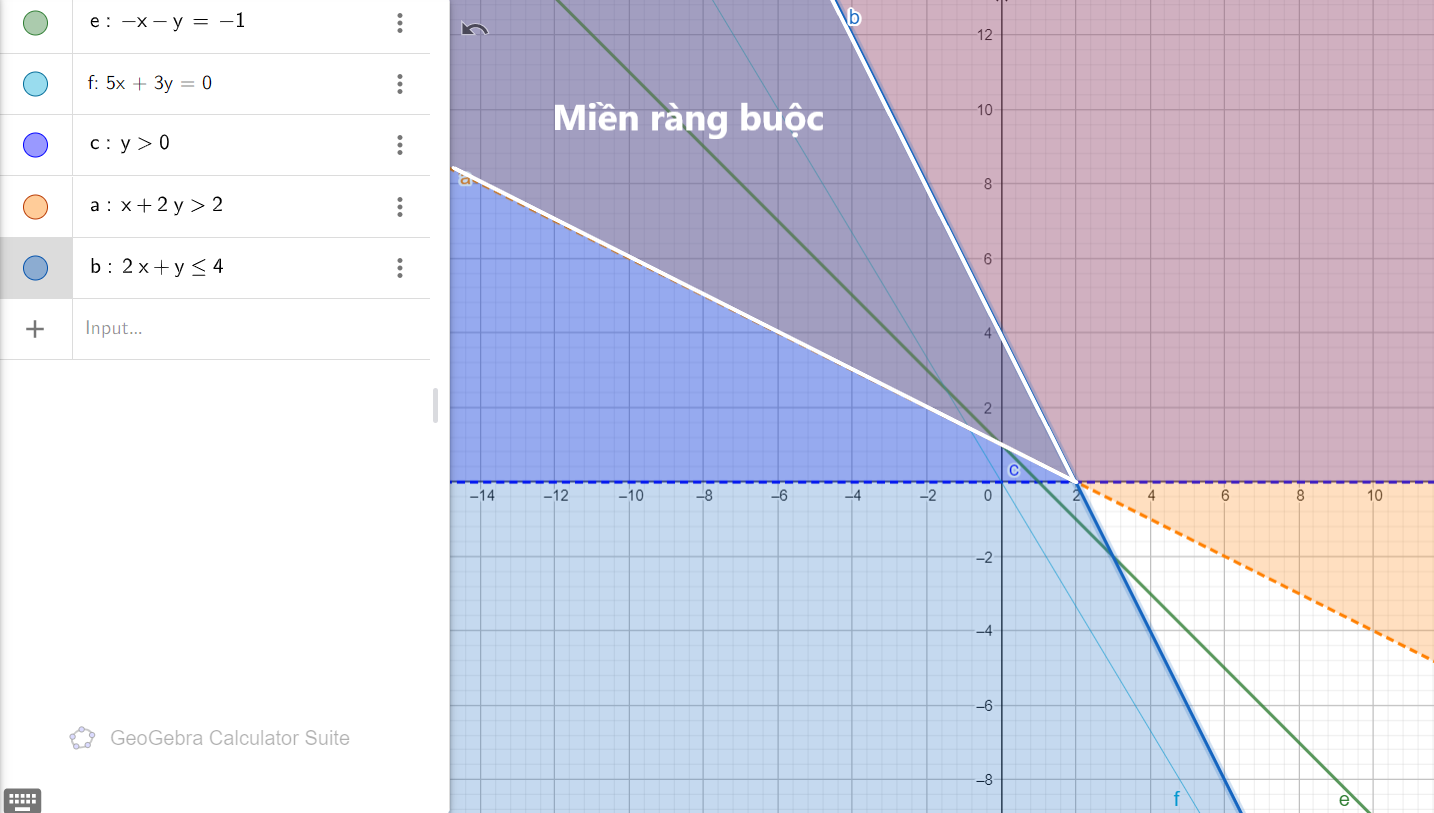
\includegraphics[scale=.4]{img/mienrangbuoc}
				\end{center}
				\caption{Miền ràng buộc cho bài toán (D)}
			\end{figure}
		\end{center}
		\subsection*{b. Người ta đã tính được phương án tối ưu của (D) ứng với hai số
0 và 1 nhưng chưa rõ giá trị nào ứng với biến nào. Không giải trực tiếp bài toán (P) hãy mô tả rõ các bước xác định phương án tối ưu cho bài toán (P) từ (D)}
			\begin{itemize}
				\item Giả sử $y_1 = 0, y_2 = 1$, thay vào điều kiện (1) của (D) $\rightarrow$ thỏa mãn, vậy $y_1 = 0, y_2 = 1$.
				\item Theo định lý độ lệch bù:
					\begin{itemize}
						\item Có $y_1 = 0$ nên không xét ràng buộc (1) của $x$.
						\item Có $y_2 = 1 \neq 0$ nên dấu = trong ràng buộc (2) của $x$ phải xảy ra, tức là $2x_1 - x_2 + x_3 = 3$.
						\item Thay bộ (0, 1) vào ràng buộc (1), (2) của $y$, thấy có dấu = xảy ra nên không xét $x_1, x_2$.
						\item Thay bộ (0, 1) vào ràng buộc (3) của $y$, thấy không có dấu = xảy ra nên $x_3 = 0$.
						\item Ta có hệ phương trình:
							\[\begin{cases}
								x_1 - x_2 + 2x_3 = 5\\
								2x_1 - x_2 + x_3 = 3\\
								x_3 = 0
							\end{cases}\]
						\item Giải hệ phương trình ta được: $x_1 = -2, x_2 = -7$, suy ra $min = 3$. 
					\end{itemize}
			\end{itemize}
	\begin{center}
		Hết./.
	\end{center}
\end{document}
